%!TeX root=../tese.tex

%% ------------------------------------------------------------------------- %%
\chapter{Conceitos básicos}
\label{cap:conceitos-basicos}

Neste capítulo serão detalhados alguns conceitos básicos relacionados ao problema
abordado e a solução proposta para endereçá-lo.

Os sistemas de software alvos desta pesquisa são sistemas de médio ou grande porte
que possuem uma arquitetura segmentada em vários serviços, visando garantir um
baixo acoplamento entre várias partes que compõe o software.

Este tipo de arquitetura inicialmente foi conhecido como SOA (mais informações em 
\emph{Service-Oriented Architecture: Concepts, Technology, and Design}~\citep{erl}),
sobre a qual serão dados mais detalhes a seguir.

\section{Sistemas com arquitetura SOA}
\label{sec:sistemas-com-arquitetura-soa}

Um sistema criado com a arquitetura SOA é um sistema modularizado em vários
serviços, em geral independentes, que em conjunto podem oferecer várias
funcionalidades a um usuário.

\begin{figure}
  \centering
  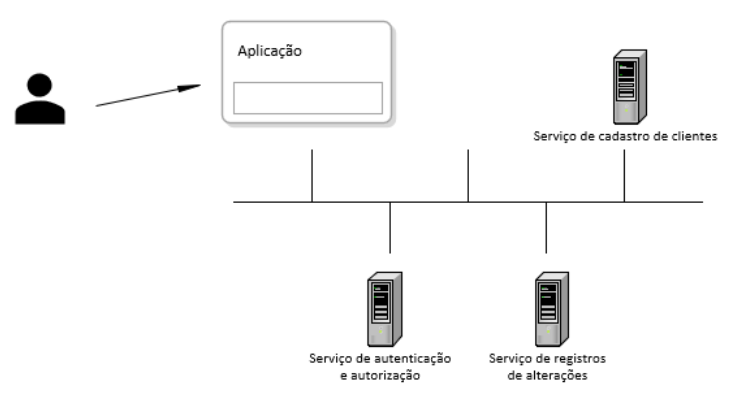
\includegraphics[width=.7\textwidth]{figura1}
  \caption{Barramento de uma aplicação SOA.\label{fig:barramento-de-uma-aplicacao-soa}}
\end{figure}

Na figura 2.1 encontra-se um diagrama simplificado de uma aplicação hipotética onde
a interface com o usuário se comunica com vários serviços como: autenticação e
autorização, cadastro de clientes e registros de alterações.

Para um usuário realizar alterações nos dados de um cliente ele irá utilizar a
interface da aplicação, que por sua vez utilizará o serviço de autenticação e
autorização para validar a identidade do usuário e se este possui as permissões
necessárias para a alteração.

Em seguida, uma chamada ao serviço de cadastro de clientes será feita para realizar
as alterações necessárias e por fim o serviço de registro de alterações será
acionado para registrar que o usuário autenticado realizou uma alteração no
cadastro de um cliente.

Com este exemplo é possível mostrar como vários serviços independentes podem ser
utilizados para compor um sistema de software modular e de baixo grau de acoplamento.

\section{Noções em escalabilidade e resiliência}
\label{sec:nocoes-em-escalabilidade-e-resiliencia}

Para que um sistema de software obtenha sucesso, ele precisa ter um grande número de
usuários, e estes precisam estar satisfeitos com seu desempenho e disponibilidade.
Estes dois requisitos não funcionais dependem de duas características do software:
escalabilidade e resiliência.

A escalabilidade se traduz na capacidade de conseguir atender desde um pequeno
número de usuários até centenas de milhares deles. Já a resiliência é caracterizada
pela capacidade do sistema de se manter operante mesmo diante de falhas, sejam estas
dentro ou fora de sua infraestrutura, que em algum momento irão ocorrer.

A escalabilidade de um sistema de software é habitualmente endereçada com a adição
de novos recursos computacionais. A adição destes recursos pode ser tanto na forma
vertical, com o aumento de recursos como processador e memória para uma instância do
sistema em execução, como horizontal, adicionando mais máquinas ao sistema.

Já a resiliência por sua vez está atrelada com a arquitetura do sistema, a qual
deverá prever que em algum momento as máquinas, conexões de rede, ou até mesmo um
\textit{data-center} inteiro poderão falhar. Com a arquitetura adequada, é possível
criar um sistema de software que atenda ambas as necessidades de escalabilidade e
resiliência.

No diagrama abaixo (figura 2.2) encontra-se um exemplo simplificado de arquitetura de
um sistema de software executado em vários servidores, os quais estão localizados
em dois \textit{data-centers} fisicamente separados, atendendo diversos usuários que
irão se conectar a estes servidores através de balanceadores de carga.

\begin{figure}
  \centering
  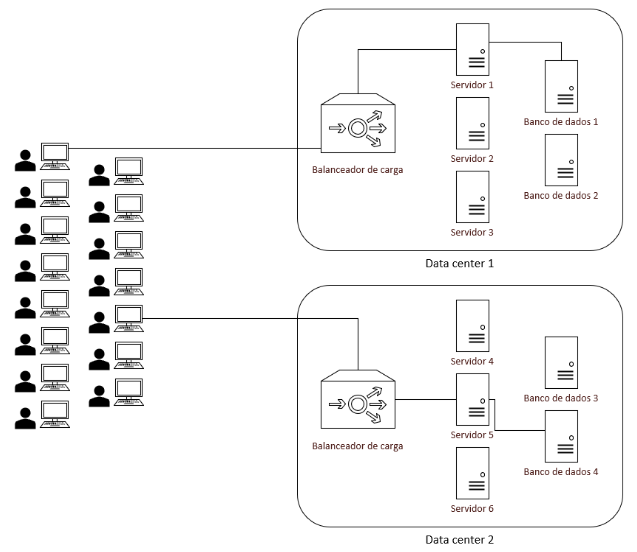
\includegraphics[width=.7\textwidth]{figura2}
  \caption{Diagrama de aplicação resiliente.\label{fig:diagrama-de-aplicacao-resiliente}}
\end{figure}

Alguns detalhes, como replicação de bancos de dados e mecanismos de direcionamento
dos usuários aos balanceadores de carga, estão ocultos nesta visualização, mas de
forma simplificada é desta maneira que um sistema de software deve ser arquitetado
para que os requisitos de escalabilidade e resiliência sejam atendidos.

\section{Balanceadores de carga}
\label{sec:balanceadores-de-carga}

Os balanceadores de carga são peças chave para que um sistema de software possa ser
escalável e resiliente (mais informações em \emph{Availability and Load Balancing in Cloud Computing}~\citep{chaczko}).
Estes componentes atuam intermediando as requisições dos usuários para os servidores,
direcionando as requisições somente para servidores que estejam em pleno funcionamento.

A resiliência é garantida pois, se um destes servidores deixar de funcionar, ele não
receberá mais requisições do balanceador de carga e também, se um dos balanceadores
de carga deixar de funcionar, um outro balanceador poderá continuar fazendo o
redirecionamento de requisições para todos os servidores ativos.

É importante notar que nunca deve haver somente um balanceador de carga, pois ele
iria comprometer totalmente a disponibilidade da aplicação em caso de falha.

\section{Micro-serviços, containers e Kubernetes}
\label{sec:micro-servicos-containers-e-kubernetes}

Com a computação em nuvem e o conceito de infraestrutura como código, o modelo de
arquitetura SOA evoluiu para o que atualmente conhecemos como micro-serviços, o
qual se diferencia principalmente pela independência na implantação de cada serviço.

O principal motivo para sua popularidade é a facilidade que cada micro-serviço
passou a ter para definição suas necessidades de servidores, balanceadores de
carga e bancos de dados, através de arquivos texto que são processados por
mecanismo de automação na sua implantação.

Na figura 2.3 é possível ver um exemplo de como uma aplicação pode ser composta de
vários micro-serviços, executados de forma independente, mas com dependências
entre si.

\begin{figure}
  \centering
  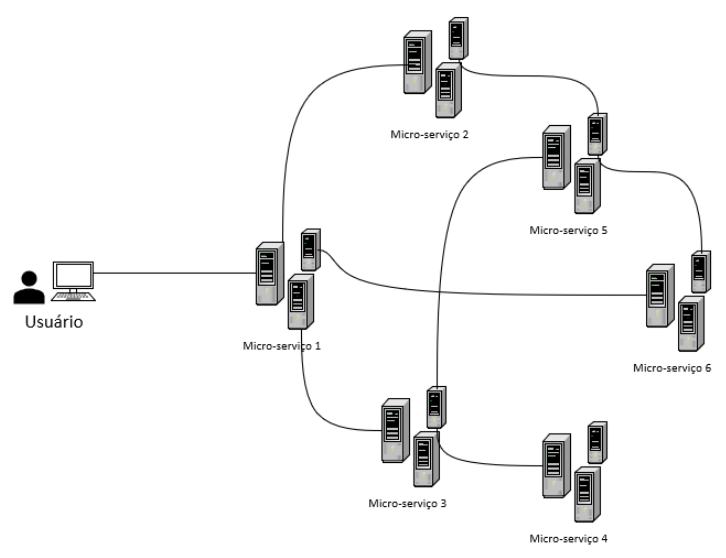
\includegraphics[width=.7\textwidth]{figura3}
  \caption{Diagrama de micro-serviços.\label{fig:diagrama-de-micro-servicos}}
\end{figure}

Como os micro-serviços que tratamos neste documento são aplicações que se
comunicam por uma rede utilizando geralmente o protocolo HTTP, estes também são
conhecidos como aplicações web.

Outro fator que posteriormente contribuiu ainda mais para a maior adoção desta
arquitetura foram os containers Linux e sistemas de orquestração e gerenciamento
de containers.

Os containers Linux permitem que um processo seja executado como se ele estivesse
em uma máquina exclusiva, isolando bibliotecas dos quais ele depende e também
oferecendo uma inicialização muito mais rápida que uma máquina virtual visto que
o núcleo do sistema operacional é compartilhado pelos vários containers e este já
está pronto para ser utilizado quando se inicia um container novo.

Para facilitar a gerência na execução de containers Linux foram criados diversos
projetos como o Kubernetes\footnote[4]{\url{http://kubernetes.io}}, desenvolvido
pela Google, e o Docker Swarm\footnote[5]{\url{docs.docker.com/engine/swarm}},
desenvolvido pela Docker Inc., também responsável pela implementação de
containers Linux denominada Docker\footnote[6]{\url{www.docker.com/resources/what-container}}.

Com a utilização destes projetos, é possível gerenciar automaticamente um conjunto
de máquinas para a execução de diversos containers de micro-serviços, garantindo
a reinicialização da aplicação em caso de falha, e escalabilidade, iniciando
novos containers nas máquinas conforme a necessidade.

\section{Detecção de falhas}
\label{sec:deteccao-de-falhas}

Para realizar uma análise de um sistema de software implantado utilizando a
arquitetura de micro-serviços, independente de sua infraestrutura de implantação,
esta pesquisa propõe uma análise não invasiva dos serviços utilizando somente os
registros dos balanceadores de carga a frente dos micro-serviços.

Os registros dos balanceadores de carga contém informações bastante interessantes
como os horários que as requisições iniciaram e foram concluídas, além de
quantidades de dados trafegados, o serviço que foi acessado e o tempo que este
serviço levou para ser executado. Estes dados devem ser suficientes para se
traçar um perfil de comportamento, permitindo detectar casos que fugiram deste
perfil e analisá-los com mais detalhes.

\section{Classificação de falhas}
\label{sec:classificacao-de-falhas}

Uma vez que as falhas podem ser detectadas, estas podem ser classificadas
conforme sua causa raiz, que pode variar desde um excesso de utilização a uma
falha de um banco de dados, por exemplo.

Com experimentos provocando falhas simuladas, é possível realizar o treinamento
de um algoritmo de aprendizado de máquina para que novas falhas de aplicações
reais possam ser classificadas, permitindo inferir a causa provável de um
problema na aplicação.

O objetivo final desta pesquisa é de detectar e classificar uma falha em um
serviço o quanto antes pois, dado o cenário complexo de micro-serviços exposto
acima, uma falha em uma aplicação pode causar impactos em outras aplicações,
o que poderia causar problemas maiores para todo o sistema de software.
